\documentclass[11pt]{article}
\usepackage[utf8]{inputenc}
\usepackage[T1]{fontenc}
\usepackage{babel}
\usepackage{graphicx}
\usepackage{xcolor}
\usepackage{listings}
\usepackage[colorlinks=true,linkcolor=blue, urlcolor=blue]{hyperref}

\lstset{
    basicstyle=\ttfamily,
    backgroundcolor=\color{lightgray},
    frame=single,
    columns=flexible
}

\date{Version Mai 2024}
\author{Valentin Gangloff
\and
Master Sécurité des Systèmes Informatiques 1ère année
\and
UFR Sciences et techniques de Rouen}
\title{Guide d'utilisation du simulateur Mermin}

\begin{document}

\maketitle

\newpage 

\tableofcontents

\newpage

\section{Présentation rapide du jeu}

Le jeu du carré de Mermin-Peres ou jeu du carré magique est un jeu à deux joueurs en un tour.
\\
Il se joue sur une grille en 3x3 :


\includegraphics[width=\textwidth]{grid.png}


\newpage 

\noindent Nous avons Alice et Bob.

\noindent Ils auront pour ordre de remplir une ligne ou une colonne avec des symboles, par exemple des "X" et des "O"
\\

\noindent Alice a une grille avec pour ordre de mettre les symboles dans une ligne qui lui sera désignée, et une contrainte qui est de mettre un nombre pair de "X" (Soit 0 ou 2)
\\

\noindent Bob aura aussi une grille, avec pour ordre de mettre des symboles dans une colonne qui lui sera désignée, avec la contrainte de mettre un nombre impair de "X" (Soit 1 ou 3)
\\

\noindent Disons que par exemple, Alice et Bob ont respectivement la ligne 1 et la colonne 2.

\noindent Ils auront donc la case centrale supérieure en commune.

\noindent S'ils mettent le même symbole dans cette case, ils ont gagné. Sinon, ils ont perdu.
\\
\newpage
\noindent Voici un exemple de victoire :
\\

\noindent Alice a rempli :


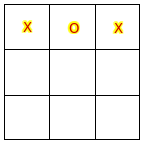
\includegraphics[width=\textwidth]{gridalice.png}

\newpage
\noindent Bob a rempli :


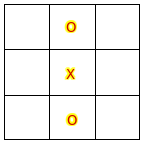
\includegraphics[width=\textwidth]{gridbob.png}

Leur case commune montre qu'ils ont le même symbole, ils ont donc gagné.

\newpage

\section{Présentation de l'appareil}

\subsection{Présentation matérielle}

L'appareil est composé de trois/quatre éléments :

\begin{itemize}
\item D'une Raspberry qui sert d'unité de contrôle et de calcul entre les deux Arduinos.
\item D'une carte Arduino avec son écran représentant Alice.
\item D'une carte Arduino avec son écran représentant Bob.
\item D'un ordinateur avec Wi-Fi pour s'interfacer avec la Raspberry pour démarrer le jeu.
\end{itemize}

\subsection{Présentation pratique}

\noindent Lors de l'allumage, la Raspberry va directement commuter en mode Hotspot pour permettre aux Arduino de se connecter dessus, les Arduino, quant à elles vont, à l'allumage tenter de se connecter au Hotspot et d'établir une connexion avec un port de la Raspberry pour démarrer le jeu. Si ces deux étapes ne sont pas faites, les écrans ne s'allumeront pas.
\\

\noindent Une fois la mise en place faite, les écrans des Arduino vont s'allumer avec l'interface de jeu, et pourront demander à la Raspberry de faire les calculs quantiques.


\newpage
\section{Mise en marche des appareils}

\subsection{La Raspberry}

Pour la mise en marche de la Raspberry, il faut, dans un premier temps, la brancher et la laisser s'initialiser.
\\

\noindent Dans un second temps, avec votre ordinateur, vous vous connecterez sur le réseau wi-fi de SSID : merminrasp, avec le mot de passe : mermin2024
\\

\noindent Une fois la connexion effectuée, vous allez lancer une connexion SSH sur le routeur de cette connexion (La Raspberry, en l'occurence), avec l'IP : 10.42.0.1
\\

\noindent Le compte utilisateur est : dptinfo et le mot de passe est : DPTInfo2024
\\

\noindent Une fois connecté, il faut tout simplement lancer le jeu. Rendez-vous dans le répertoire du jeu nommé ProjetIQ et deux choix s'offrent à vous.
\\

\noindent Soit vous lancez le script python tel quel et vous aurez des retours console pour s'assurer que tout va bien 

\begin{lstlisting}[language=bash]
	python3 controller.py
\end{lstlisting}

\noindent Soit vous lancez le script bash qui permet d'éliminer les retours console, pour permettre de couper la connexion SSH et laisser la Raspberry se débrouiller toute seule

\begin{lstlisting}[language=bash]
	bash launch.sh
\end{lstlisting}

\noindent Ce script est une simple commande nohup, mais il est là si vous avez le désir de tout automatiser au démarrage de l'OS de la Raspberry :

\begin{lstlisting}[language=bash]
	nohup python3 controller.py
\end{lstlisting}

\noindent Une fois tout cela fait, vous n'avez plus besoin d'interagir avec la Raspberry

\newpage
\subsection{Les Arduino}

\noindent Pour mettre en place les Arduino, il faut d'abord préparer la Raspberry, comme explicité dans la section précédente.
\\

\noindent Lors de la mise sous tension de l'Arduino, cette dernière va chercher à se connecter au Hotspot puis, au port ouvert par la Raspberry. L'écran s'illuminera au moment où la connexion sera effectuée. Si au bout de 20 sec, l'écran ne s'allume toujours pas, il suffit d'appuyer sur l'un des deux boutons Reset situés sur l'Arduino ou sur le Shield de l'Arduino.
\\

\noindent Une fois cela fait, les Arduino sont faites pour fonctionner de façon autonome.

\newpage 
\section{Présentation de l'interface}

\subsection{Interface de jeu}

L'interface de jeu qui est aussi l'interface affichée au démarrage est la suivante :

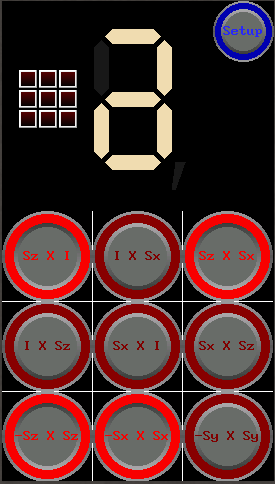
\includegraphics[]{Interface1.png}

\begin{itemize}
\item Le chiffre central sera le résultat de la mesure effectuée.
\item La petite matrice à gauche du chiffre s'illumine pour montrer quelle mesure a été déjà faite, et donc quelle case de la grille a été mesurée.
\item Les neuf boutons représente les neufs mesures pouvant être faites et surtout, par association, quelle case on mesure.
\item Le bouton setup permet d'accéder au menu pour des options supplémentaires.
\end{itemize}

\subsection{Interface de configuration}

L'interface de configuration permet d'avoir des options supplémentaires, et d'identifier l'appareil en question :

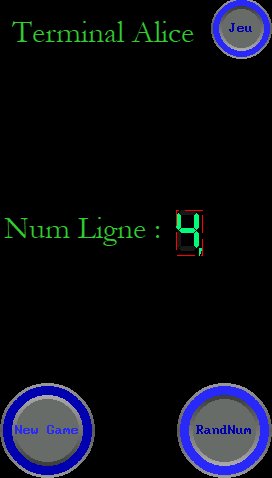
\includegraphics[]{Interface2.png}

\begin{itemize}
	\item Le bouton New Game permet de relancer une nouvelle instance du jeu pour les deux appareils 
	\item Le bouton RandNum permet de générer un nombre aléatoire pour la ligne ou la colonne pour éviter d'avoir à tirer nous-même les nombres pour associer les lignes et colonnes à Alice ou Bob.
	\item Le bouton Jeu permet de revenir à l'interface du jeu.
\end{itemize}

\end{document}